% LESSON 2: ANGLES IN STANDARD POSITION

\documentclass[aspectratio=169]{beamer}
\usepackage{amsmath}
\usepackage{amssymb}
\usepackage{graphicx}
\usepackage{tcolorbox}
\usepackage{booktabs}
\usepackage{colortbl}
\usepackage{xcolor}
\usepackage{tikz}
\usetikzlibrary{angles,quotes}
\usepackage[utf8]{inputenc}

% Custom colors
\definecolor{primary}{RGB}{41, 128, 185}
\definecolor{secondary}{RGB}{52, 152, 219}
\definecolor{accent}{RGB}{231, 76, 60}
\definecolor{lightgray}{RGB}{236, 240, 241}

% Theme customization
\usetheme{Madrid}
\usecolortheme{whale}
\setbeamercolor{structure}{fg=primary}
\setbeamercolor{background canvas}{bg=white}
\setbeamercolor{normal text}{fg=black}

% Title page info
\title{Pre-Calculus 11}
\subtitle{Lesson 2: Angles in Standard Position}
\author{Created by Yi-Chen Lin}
\date{\today}

\begin{document}

\begin{frame}
    \titlepage
    \vfill
    \centering
\end{frame}

% I) NAMING QUADRANTS & X/Y AXIS
\begin{frame}{Naming Quadrants \\& X/Y Axis}
    \begin{tcolorbox}[colback=lightgray,colframe=primary,title=Quadrants and Axes]
        \footnotesize
        \begin{columns}
            \column{0.6\textwidth}
            \begin{itemize}
                \item There are Four Quadrants in the XY plane
                \item On the X-axis: Right – Positive, Left - Negative
                \item On the Y-axis: Up – Positive, Bottom - Negative
                \item Center: Origin (0,0)
            \end{itemize}
            \begin{center}
            \begin{tabular}{|c|c|c|}
            \hline
            Quadrant & X Coordinates & Y Coordinates \\
            \hline
            1 & + & + \\
            2 & - & + \\
            3 & - & - \\
            4 & + & - \\
            \hline
            \end{tabular}
            \end{center}
            \column{0.4\textwidth}
            % Quadrant diagram placeholder
            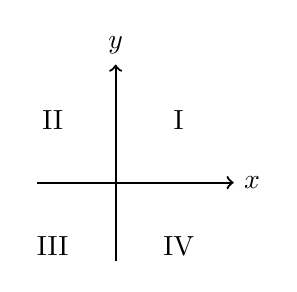
\begin{tikzpicture}[scale=1]
                \draw[thick,->] (-1,0) -- (1.5,0) node[right]{$x$};
                \draw[thick,->] (0,-1) -- (0,1.5) node[above]{$y$};
                \node at (0.8,0.8) {I};
                \node at (-0.8,0.8) {II};
                \node at (-0.8,-0.8) {III};
                \node at (0.8,-0.8) {IV};
            \end{tikzpicture}
        \end{columns}
    \end{tcolorbox}
\end{frame}

% II) ANGLES IN STANDARD POSITION - CONTENT
\begin{frame}{II) Angles in Standard Position}
    \begin{tcolorbox}[colback=lightgray,colframe=primary,title=Angles in Standard Position]
        \footnotesize
        \begin{itemize}
            \item Drawing an angle in standard position means that you start from the right side of the X-axis at 0 degrees
            \item When drawing the angle, indicate which direction it is rotating: Clockwise (Positive) and Counter Clockwise (Negative)
            \item The initial arm is the positive side of the X-axis
            \item The terminal arm is the line that rotates around the origin, with a radius of 1 (UNIT CIRCLE)
        \end{itemize}
    \end{tcolorbox}
\end{frame}

% II) ANGLES IN STANDARD POSITION - TIKZ DIAGRAM
\begin{frame}{II) Angles in Standard Position (Diagram)}
\centering
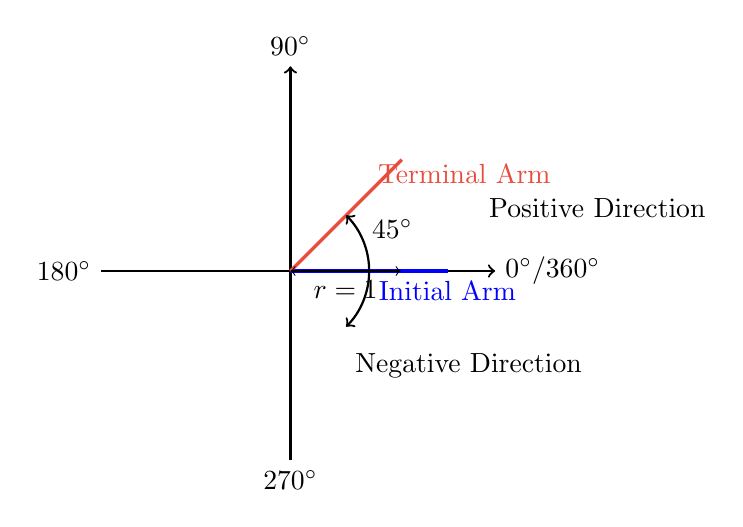
\begin{tikzpicture}[scale=2]
  % Draw axes
  \draw[thick,->] (-1.2,0) -- (1.3,0) node[right] {$0^\circ$/$360^\circ$};
  \draw[thick,->] (0,-1.2) -- (0,1.3) node[above] {$90^\circ$};
  \draw[thick] (-1,0) -- (-1.2,0) node[left] {$180^\circ$};
  \draw[thick] (0,-1) -- (0,-1.2) node[below] {$270^\circ$};

  % Initial arm
  \draw[very thick,blue] (0,0) -- (1,0);
  \node[below right,blue] at (0.5,0) {Initial Arm};

  % Terminal arm (example: 45 degrees)
  \draw[very thick,accent] (0,0) -- ({cos(45)},{sin(45)});
  \node[above right,accent] at ({0.7*cos(45)},{0.7*sin(45)}) {Terminal Arm};

  % Arc for positive direction
  \draw[->,thick] (0.5,0) arc (0:45:0.5);
  \node[right] at (1.2,0.4) {Positive Direction};

  % Arc for negative direction
  \draw[->,thick] (0.5,0) arc (0:-45:0.5);
  \node[right] at (0.35,-0.6) {Negative Direction};

  % Radius label
  \draw[<->] (0,0) -- (0.7,0);
  \node[below] at (0.35,0) {$r=1$};

  % Angle label
  \node at ({0.7*cos(22.5)},{0.7*sin(22.5)}) {$45^\circ$};
\end{tikzpicture}
\end{frame}

% III) DRAWING ANGLES IN STANDARD POSITION - CONTENT
\begin{frame}{III) Drawing Angles in Standard Position}
    \begin{tcolorbox}[colback=lightgray,colframe=primary,title=Drawing Angles in Standard Position]
        \footnotesize
        \begin{itemize}
            \item When drawing angles in "standard position" make sure they begin at the Initial arm at $0^\circ$
            \item Draw the Terminal arm in the quadrant, approximate it
            \item Make sure you draw the curve indicating the direction and number of rotations
        \end{itemize}
    \end{tcolorbox}
\end{frame}

% III) DRAWING ANGLES IN STANDARD POSITION - EXAMPLES (62°, 152°)
\begin{frame}{III) Drawing Angles in Standard Position: Examples}
\centering
\begin{columns}
  \column{0.5\textwidth}
  \textbf{a) $62^\circ$}
  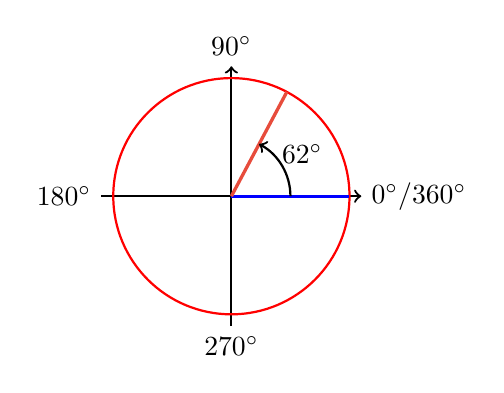
\begin{tikzpicture}[scale=1.5]
    % Axes
    \draw[thick,->] (-1.1,0) -- (1.1,0) node[right] {$0^\circ$/$360^\circ$};
    \draw[thick,->] (0,-1.1) -- (0,1.1) node[above] {$90^\circ$};
    \draw[thick] (-1,0) -- (-1.1,0) node[left] {$180^\circ$};
    \draw[thick] (0,-1) -- (0,-1.1) node[below] {$270^\circ$};
    % Circle
    \draw[thick,red] (0,0) circle(1);
    % Initial arm
    \draw[very thick,blue] (0,0) -- (1,0);
    % Terminal arm
    \draw[very thick,accent] (0,0) -- ({cos(62)},{sin(62)});
    % Arc
    \draw[->,thick] (0.5,0) arc (0:62:0.5);
    % Angle label
    \node at ({0.7*cos(31)},{0.7*sin(31)}) {$62^\circ$};
  \end{tikzpicture}
  \column{0.5\textwidth}
  \textbf{b) $152^\circ$}
  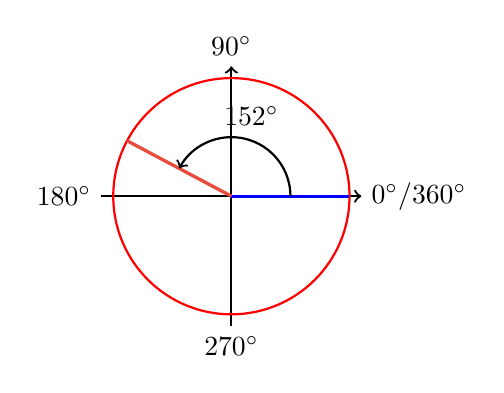
\begin{tikzpicture}[scale=1.5]
    % Axes
    \draw[thick,->] (-1.1,0) -- (1.1,0) node[right] {$0^\circ$/$360^\circ$};
    \draw[thick,->] (0,-1.1) -- (0,1.1) node[above] {$90^\circ$};
    \draw[thick] (-1,0) -- (-1.1,0) node[left] {$180^\circ$};
    \draw[thick] (0,-1) -- (0,-1.1) node[below] {$270^\circ$};
    % Circle
    \draw[thick,red] (0,0) circle(1);
    % Initial arm
    \draw[very thick,blue] (0,0) -- (1,0);
    % Terminal arm
    \draw[very thick,accent] (0,0) -- ({cos(152)},{sin(152)});
    % Arc
    \draw[->,thick] (0.5,0) arc (0:152:0.5);
    % Angle label
    \node at ({0.7*cos(76)},{0.7*sin(76)}) {$152^\circ$};
  \end{tikzpicture}
\end{columns}
\end{frame}

% III) DRAWING ANGLES IN STANDARD POSITION - MORE EXAMPLES (312°, -77°)
\begin{frame}{III) Drawing Angles in Standard Position: More Examples}
\centering
\begin{columns}
  \column{0.5\textwidth}
  \textbf{c) $312^\circ$}
  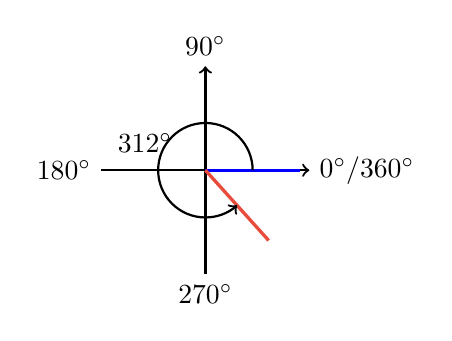
\begin{tikzpicture}[scale=1.2]
    \draw[thick,->] (-1.1,0) -- (1.1,0) node[right] {$0^\circ$/$360^\circ$};
    \draw[thick,->] (0,-1.1) -- (0,1.1) node[above] {$90^\circ$};
    \draw[thick] (-1,0) -- (-1.1,0) node[left] {$180^\circ$};
    \draw[thick] (0,-1) -- (0,-1.1) node[below] {$270^\circ$};
    %\draw[thick,red] (0,0) circle(1);
    \draw[very thick,blue] (0,0) -- (1,0);
    \draw[very thick,accent] (0,0) -- ({cos(312)},{sin(312)});
    \draw[->,thick] (0.5,0) arc (0:312:0.5);
    \node at ({0.7*cos(156)},{0.7*sin(156)}) {$312^\circ$};
  \end{tikzpicture}
  \column{0.5\textwidth}
  \textbf{d) $-77^\circ$}
  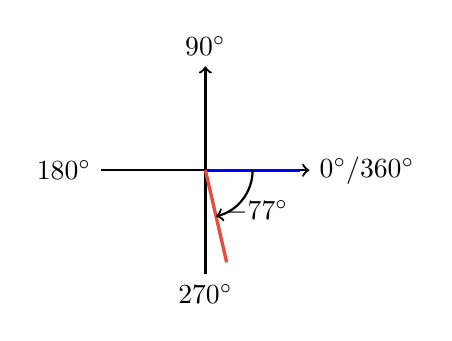
\begin{tikzpicture}[scale=1.2]
    \draw[thick,->] (-1.1,0) -- (1.1,0) node[right] {$0^\circ$/$360^\circ$};
    \draw[thick,->] (0,-1.1) -- (0,1.1) node[above] {$90^\circ$};
    \draw[thick] (-1,0) -- (-1.1,0) node[left] {$180^\circ$};
    \draw[thick] (0,-1) -- (0,-1.1) node[below] {$270^\circ$};
    %\draw[thick,red] (0,0) circle(1);
    \draw[very thick,blue] (0,0) -- (1,0);
    \draw[very thick,accent] (0,0) -- ({cos(-77)},{sin(-77)});
    \draw[->,thick] (0.5,0) arc (0:-77:0.5);
    \node at ({0.7*cos(-38.5)},{0.7*sin(-38.5)}) {$-77^\circ$};
  \end{tikzpicture}
\end{columns}
\end{frame}

% III) DRAWING ANGLES IN STANDARD POSITION - EVEN MORE EXAMPLES (450°, 540°)
\begin{frame}{III) Drawing Angles in Standard Position: Even More Examples}
\centering
\begin{columns}
  \column{0.5\textwidth}
  \textbf{e) $450^\circ$}
  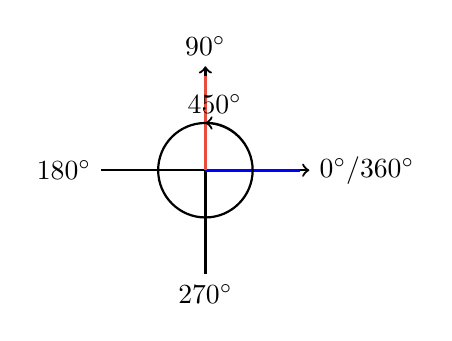
\begin{tikzpicture}[scale=1.2]
    \draw[thick,->] (-1.1,0) -- (1.1,0) node[right] {$0^\circ$/$360^\circ$};
    \draw[thick,->] (0,-1.1) -- (0,1.1) node[above] {$90^\circ$};
    \draw[thick] (-1,0) -- (-1.1,0) node[left] {$180^\circ$};
    \draw[thick] (0,-1) -- (0,-1.1) node[below] {$270^\circ$};
    %\draw[thick,red] (0,0) circle(1);
    \draw[very thick,blue] (0,0) -- (1,0);
    \draw[very thick,accent] (0,0) -- (0,1);
    \draw[->,thick] (0.5,0) arc (0:450:0.5);
    \node at (0.1,0.7) {$450^\circ$};
  \end{tikzpicture}
  \column{0.5\textwidth}
  \textbf{f) $540^\circ$}
  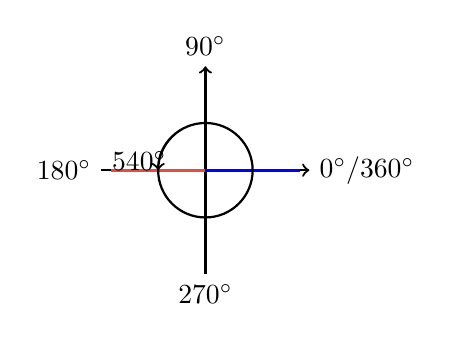
\begin{tikzpicture}[scale=1.2]
    \draw[thick,->] (-1.1,0) -- (1.1,0) node[right] {$0^\circ$/$360^\circ$};
    \draw[thick,->] (0,-1.1) -- (0,1.1) node[above] {$90^\circ$};
    \draw[thick] (-1,0) -- (-1.1,0) node[left] {$180^\circ$};
    \draw[thick] (0,-1) -- (0,-1.1) node[below] {$270^\circ$};
    %\draw[thick,red] (0,0) circle(1);
    \draw[very thick,blue] (0,0) -- (1,0);
    \draw[very thick,accent] (0,0) -- (-1,0);
    \draw[->,thick] (0.5,0) arc (0:540:0.5);
    \node at (-0.7,0.1) {$540^\circ$};
  \end{tikzpicture}
\end{columns}
\end{frame}

% IV) CO-TERMINAL ANGLES - CONTENT
\begin{frame}{IV) Co-terminal Angles}
    \begin{tcolorbox}[colback=lightgray,colframe=primary,title=Co-terminal Angles]
        \footnotesize
        \begin{itemize}
            \item Two angles are called "co-terminal" if they are located at the same position
            \item Co-terminal angles have a difference of $360^\circ$ or multiples of $360^\circ$ (Full circles)
            \item These angles are co-terminal with each other: $30^\circ$, $390^\circ$, $750^\circ$, $-330^\circ$, $-690^\circ$, etc.
        \end{itemize}
    \end{tcolorbox}
\end{frame}

% IV) CO-TERMINAL ANGLES - SINGLE DIAGRAMS

\begin{frame}{IV) Co-terminal Angle: $30^\circ$}
\centering
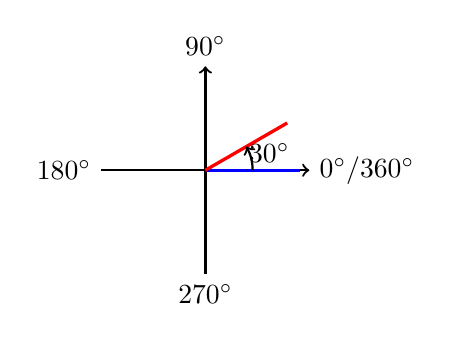
\begin{tikzpicture}[scale=1.2]
  % Axes
  \draw[thick,->] (-1.1,0) -- (1.1,0) node[right] {$0^\circ$/$360^\circ$};
  \draw[thick,->] (0,-1.1) -- (0,1.1) node[above] {$90^\circ$};
  \draw[thick] (-1,0) -- (-1.1,0) node[left] {$180^\circ$};
  \draw[thick] (0,-1) -- (0,-1.1) node[below] {$270^\circ$};
  % Initial arm
  \draw[very thick,blue] (0,0) -- (1,0);
  % Terminal arm (30°)
  \draw[very thick,red] (0,0) -- ({cos(30)},{sin(30)});
  % Arc
  \draw[->,thick] (0.5,0) arc (0:30:0.5);
  % Angle label
  \node at ({0.7*cos(15)},{0.7*sin(15)}) {$30^\circ$};
\end{tikzpicture}
\end{frame}

\begin{frame}{IV) Co-terminal Angle: $390^\circ$}
\centering
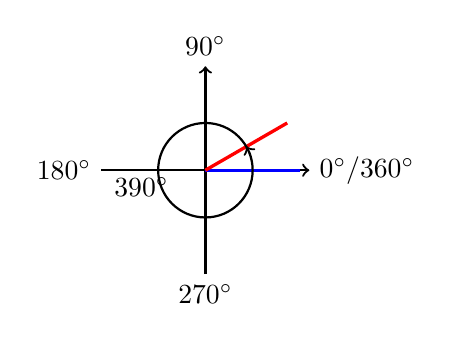
\begin{tikzpicture}[scale=1.2]
  % Axes
  \draw[thick,->] (-1.1,0) -- (1.1,0) node[right] {$0^\circ$/$360^\circ$};
  \draw[thick,->] (0,-1.1) -- (0,1.1) node[above] {$90^\circ$};
  \draw[thick] (-1,0) -- (-1.1,0) node[left] {$180^\circ$};
  \draw[thick] (0,-1) -- (0,-1.1) node[below] {$270^\circ$};
  % Initial arm
  \draw[very thick,blue] (0,0) -- (1,0);
  % Terminal arm (390°)
  \draw[very thick,red] (0,0) -- ({cos(390)},{sin(390)});
  % Arc
  \draw[->,thick] (0.5,0) arc (0:390:0.5);
  % Angle label
  \node at ({0.7*cos(195)},{0.7*sin(195)}) {$390^\circ$};
\end{tikzpicture}
\end{frame}

\begin{frame}{IV) Co-terminal Angle: $-330^\circ$}
\centering
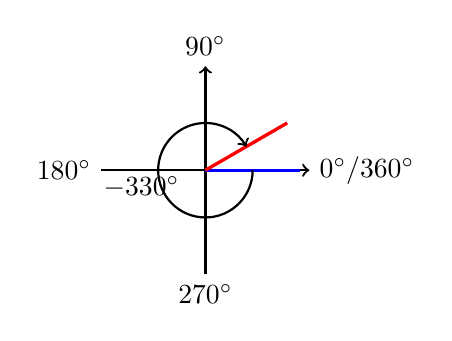
\begin{tikzpicture}[scale=1.2]
  % Axes
  \draw[thick,->] (-1.1,0) -- (1.1,0) node[right] {$0^\circ$/$360^\circ$};
  \draw[thick,->] (0,-1.1) -- (0,1.1) node[above] {$90^\circ$};
  \draw[thick] (-1,0) -- (-1.1,0) node[left] {$180^\circ$};
  \draw[thick] (0,-1) -- (0,-1.1) node[below] {$270^\circ$};
  % Initial arm
  \draw[very thick,blue] (0,0) -- (1,0);
  % Terminal arm (-330°)
  \draw[very thick,red] (0,0) -- ({cos(-330)},{sin(-330)});
  % Arc
  \draw[->,thick] (0.5,0) arc (0:-330:0.5);
  % Angle label
  \node at ({0.7*cos(-165)},{0.7*sin(-165)}) {$-330^\circ$};
\end{tikzpicture}
\end{frame}

% V) REFERENCE ANGLES
\begin{frame}{Reference Angles}
    \begin{tcolorbox}[colback=lightgray,colframe=primary,title=Reference Angles]
        \footnotesize
        \begin{columns}
            \column{0.6\textwidth}
            \begin{itemize}
                \item Reference angle: angle between terminal arm and x-axis
                \item Must be in the same quadrant as the terminal arm
                \item Used for SINE, COSINE, TANGENT of angles $>90^\circ$
            \end{itemize}
            \begin{itemize}
                \item Ex: $152^\circ$ reference: $180^\circ - 152^\circ = 28^\circ$
                \item Ex: $255^\circ$ reference: $255^\circ - 180^\circ = 75^\circ$
                \item Ex: $420^\circ$ reference: $420^\circ - 360^\circ = 60^\circ$
                \item Ex: $-388^\circ$ reference: $388^\circ - 360^\circ = 28^\circ$
            \end{itemize}
            \column{0.4\textwidth}
            % Reference angle diagram
            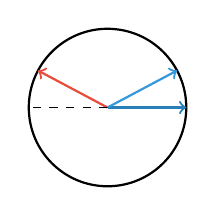
\begin{tikzpicture}[scale=1]
                \draw[thick] (0,0) circle(1);
                \draw[thick,->,primary] (0,0) -- (1,0);
                \draw[thick,->,accent] (0,0) -- ({cos(152)},{sin(152)});
                \draw[dashed] (0,0) -- ({cos(180)},{sin(180)});
                \draw[thick,->,secondary] (0,0) -- ({cos(28)},{sin(28)});
            \end{tikzpicture}
        \end{columns}
    \end{tcolorbox}
\end{frame}

% V) REFERENCE ANGLES - EXAMPLES

\begin{frame}{V) Reference Angle Example: $152^\circ$}
\centering
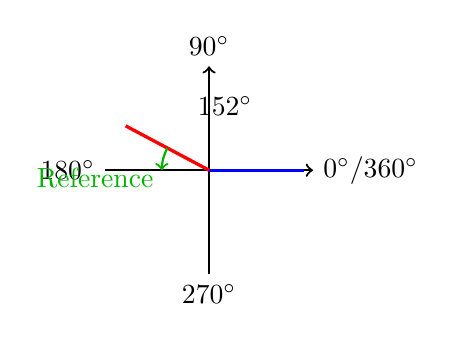
\begin{tikzpicture}[scale=1.2]
  % Axes
  \draw[thick,->] (-1.1,0) -- (1.1,0) node[right] {$0^\circ$/$360^\circ$};
  \draw[thick,->] (0,-1.1) -- (0,1.1) node[above] {$90^\circ$};
  \draw[thick] (-1,0) -- (-1.1,0) node[left] {$180^\circ$};
  \draw[thick] (0,-1) -- (0,-1.1) node[below] {$270^\circ$};
  % Initial arm
  \draw[very thick,blue] (0,0) -- (1,0);
  % Terminal arm (152°)
  \draw[very thick,red] (0,0) -- ({cos(152)},{sin(152)});
  % Reference angle arc (green)
  \draw[->,thick,green!70!black] ({0.5*cos(152)},{0.5*sin(152)}) arc (152:180:0.5);
  % Angle labels
  \node at ({0.7*cos(76)},{0.7*sin(76)}) {$152^\circ$};
  \node[green!70!black,below left] at ({0.5*cos(166)},{0.5*sin(166)}) {Reference};
\end{tikzpicture}
\end{frame}

\begin{frame}{V) Reference Angle Example: $255^\circ$}
\centering
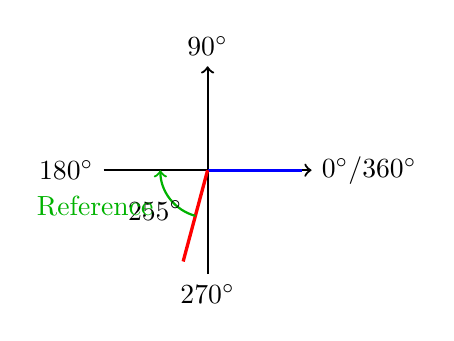
\begin{tikzpicture}[scale=1.2]
  % Axes
  \draw[thick,->] (-1.1,0) -- (1.1,0) node[right] {$0^\circ$/$360^\circ$};
  \draw[thick,->] (0,-1.1) -- (0,1.1) node[above] {$90^\circ$};
  \draw[thick] (-1,0) -- (-1.1,0) node[left] {$180^\circ$};
  \draw[thick] (0,-1) -- (0,-1.1) node[below] {$270^\circ$};
  % Initial arm
  \draw[very thick,blue] (0,0) -- (1,0);
  % Terminal arm (255°)
  \draw[very thick,red] (0,0) -- ({cos(255)},{sin(255)});
  % Reference angle arc (green)
  \draw[->,thick,green!70!black] ({0.5*cos(255)},{0.5*sin(255)}) arc (255:180:0.5);
  % Angle labels
  \node at ({0.7*cos(217.5)},{0.7*sin(217.5)}) {$255^\circ$};
  \node[green!70!black,below left] at ({0.5*cos(200)},{0.5*sin(200)}) {Reference};
\end{tikzpicture}
\end{frame}

% V) REFERENCE ANGLES - PRACTICE PROBLEMS (SPLIT)

% a) 123°
\begin{frame}{V) Reference Angles: Practice (a)}
\begin{tcolorbox}[colback=lightgray,colframe=accent,title=Practice: Find the Reference Angle]
\footnotesize
Draw $123^\circ$ in standard position and find its reference angle.

\vspace{1em}

\textbf{Blank Axis:}

\begin{center}
\begin{tikzpicture}[scale=1.1]
  \draw[thick,->] (-1.1,0) -- (1.1,0) node[right] {$0^\circ$/$360^\circ$};
  \draw[thick,->] (0,-1.1) -- (0,1.1) node[above] {$90^\circ$};
  \draw[thick] (-1,0) -- (-1.1,0) node[left] {$180^\circ$};
  \draw[thick] (0,-1) -- (0,-1.1) node[below] {$270^\circ$};
\end{tikzpicture}
\end{center}
\end{tcolorbox}
\end{frame}

% b) -210°
\begin{frame}{V) Reference Angles: Practice (b)}
\begin{tcolorbox}[colback=lightgray,colframe=accent,title=Practice: Find the Reference Angle]
\footnotesize
Draw $-210^\circ$ in standard position and find its reference angle.

\vspace{1em}

\textbf{Blank Axis:}

\begin{center}
\begin{tikzpicture}[scale=1.1]
  \draw[thick,->] (-1.1,0) -- (1.1,0) node[right] {$0^\circ$/$360^\circ$};
  \draw[thick,->] (0,-1.1) -- (0,1.1) node[above] {$90^\circ$};
  \draw[thick] (-1,0) -- (-1.1,0) node[left] {$180^\circ$};
  \draw[thick] (0,-1) -- (0,-1.1) node[below] {$270^\circ$};
\end{tikzpicture}
\end{center}
\end{tcolorbox}
\end{frame}

% c) 370°
\begin{frame}{V) Reference Angles: Practice (c)}
\begin{tcolorbox}[colback=lightgray,colframe=accent,title=Practice: Find the Reference Angle]
\footnotesize
Draw $370^\circ$ in standard position and find its reference angle.

\vspace{1em}

\textbf{Blank Axis:}

\begin{center}
\begin{tikzpicture}[scale=1.1]
  \draw[thick,->] (-1.1,0) -- (1.1,0) node[right] {$0^\circ$/$360^\circ$};
  \draw[thick,->] (0,-1.1) -- (0,1.1) node[above] {$90^\circ$};
  \draw[thick] (-1,0) -- (-1.1,0) node[left] {$180^\circ$};
  \draw[thick] (0,-1) -- (0,-1.1) node[below] {$270^\circ$};
\end{tikzpicture}
\end{center}
\end{tcolorbox}
\end{frame}

% d) -480°
\begin{frame}{V) Reference Angles: Practice (d)}
\begin{tcolorbox}[colback=lightgray,colframe=accent,title=Practice: Find the Reference Angle]
\footnotesize
Draw $-480^\circ$ in standard position and find its reference angle.

\vspace{1em}

\textbf{Blank Axis:}

\begin{center}
\begin{tikzpicture}[scale=1.1]
  \draw[thick,->] (-1.1,0) -- (1.1,0) node[right] {$0^\circ$/$360^\circ$};
  \draw[thick,->] (0,-1.1) -- (0,1.1) node[above] {$90^\circ$};
  \draw[thick] (-1,0) -- (-1.1,0) node[left] {$180^\circ$};
  \draw[thick] (0,-1) -- (0,-1.1) node[below] {$270^\circ$};
\end{tikzpicture}
\end{center}
\end{tcolorbox}
\end{frame}

% V) REFERENCE ANGLES - PRACTICE (PART 2)
\begin{frame}{V) Reference Angles: Practice (More)}
\begin{tcolorbox}[colback=lightgray,colframe=accent,title=Practice]
\footnotesize
Find the reference angle for each: $240^\circ$, $-225^\circ$, $150^\circ$, $432^\circ$
\end{tcolorbox}
\end{frame}

\begin{frame}{V) Reference Angles: Practice (Same Reference)}
\begin{tcolorbox}[colback=lightgray,colframe=accent,title=Practice]
\footnotesize
Which of the following have the same reference angle: $195^\circ$, $285^\circ$, $165^\circ$, $345^\circ$, $-15^\circ$, $105^\circ$, $85^\circ$, $-735^\circ$
\end{tcolorbox}
\end{frame}

% APPLICATION
\begin{frame}{Application: Sine, Cosine, Tangent}
    \begin{tcolorbox}[colback=lightgray,colframe=primary,title=Application]
        \footnotesize
        \begin{itemize}
            \item If you want to SINE, COSINE, or TANGENT an angle greater than $90^\circ$, use the reference angle
            \item Example: Find $\sin 195^\circ$
            \item Step 1: Make a right triangle with the reference angle
            \item Step 2: Indicate what the "opp", "adj" and "hyp" sides are
            \item Note: UP/RIGHT (Positive), DOWN/LEFT (Negative), Hypotenuse is always positive
        \end{itemize}
    \end{tcolorbox}
\end{frame}

% APPLICATION PRACTICE: STANDARD ANGLE DRAWING (3 QUESTIONS)

% Q1
\begin{frame}{Application Practice: Standard Angle (a)}
\begin{tcolorbox}[colback=lightgray,colframe=primary,title=Practice: Draw the Angle]
\footnotesize
Draw $117^\circ$ in standard position.

\vspace{1em}
\textbf{Blank Axis:}
\begin{center}
\begin{tikzpicture}[scale=1.1]
  \draw[thick,->] (-1.1,0) -- (1.1,0) node[right] {$0^\circ$/$360^\circ$};
  \draw[thick,->] (0,-1.1) -- (0,1.1) node[above] {$90^\circ$};
  \draw[thick] (-1,0) -- (-1.1,0) node[left] {$180^\circ$};
  \draw[thick] (0,-1) -- (0,-1.1) node[below] {$270^\circ$};
\end{tikzpicture}
\end{center}
\end{tcolorbox}
\end{frame}

% Q2
\begin{frame}{Application Practice: Standard Angle (b)}
\begin{tcolorbox}[colback=lightgray,colframe=primary,title=Practice: Draw the Angle]
\footnotesize
Draw $-240^\circ$ in standard position.

\vspace{1em}
\textbf{Blank Axis:}
\begin{center}
\begin{tikzpicture}[scale=1.1]
  \draw[thick,->] (-1.1,0) -- (1.1,0) node[right] {$0^\circ$/$360^\circ$};
  \draw[thick,->] (0,-1.1) -- (0,1.1) node[above] {$90^\circ$};
  \draw[thick] (-1,0) -- (-1.1,0) node[left] {$180^\circ$};
  \draw[thick] (0,-1) -- (0,-1.1) node[below] {$270^\circ$};
\end{tikzpicture}
\end{center}
\end{tcolorbox}
\end{frame}

% Q3
\begin{frame}{Application Practice: Standard Angle (c)}
\begin{tcolorbox}[colback=lightgray,colframe=primary,title=Practice: Draw the Angle]
\footnotesize
Draw $315^\circ$ in standard position.

\vspace{1em}
\textbf{Blank Axis:}
\begin{center}
\begin{tikzpicture}[scale=1.1]
  \draw[thick,->] (-1.1,0) -- (1.1,0) node[right] {$0^\circ$/$360^\circ$};
  \draw[thick,->] (0,-1.1) -- (0,1.1) node[above] {$90^\circ$};
  \draw[thick] (-1,0) -- (-1.1,0) node[left] {$180^\circ$};
  \draw[thick] (0,-1) -- (0,-1.1) node[below] {$270^\circ$};
\end{tikzpicture}
\end{center}
\end{tcolorbox}
\end{frame}

% APPLICATION PRACTICE: REFERENCE ANGLE APPLICATION (5 QUESTIONS)

% Q1
\begin{frame}{Application: Sine, Cosine, Tangent (a)}
\begin{tcolorbox}[colback=lightgray,colframe=primary,title=Application]
\footnotesize
Find $\sin 225^\circ$ by using its reference angle.\
Step 1: Make a right triangle with the reference angle.\\
Step 2: Indicate what the "opp", "adj" and "hyp" sides are.\\
Note: UP/RIGHT (Positive), DOWN/LEFT (Negative), Hypotenuse is always positive.

\vspace{1em}
\textbf{Blank Axis:}
\begin{center}
\begin{tikzpicture}[scale=1.1]
  \draw[thick,->] (-1.1,0) -- (1.1,0) node[right] {$0^\circ$/$360^\circ$};
  \draw[thick,->] (0,-1.1) -- (0,1.1) node[above] {$90^\circ$};
  \draw[thick] (-1,0) -- (-1.1,0) node[left] {$180^\circ$};
  \draw[thick] (0,-1) -- (0,-1.1) node[below] {$270^\circ$};
\end{tikzpicture}
\end{center}
\end{tcolorbox}
\end{frame}

% Q2
\begin{frame}{Application: Sine, Cosine, Tangent (b)}
\begin{tcolorbox}[colback=lightgray,colframe=primary,title=Application]
\footnotesize
Find $\cos 315^\circ$ by using its reference angle.\
Step 1: Make a right triangle with the reference angle.\\
Step 2: Indicate what the "opp", "adj" and "hyp" sides are.\\
Note: UP/RIGHT (Positive), DOWN/LEFT (Negative), Hypotenuse is always positive.

\vspace{1em}
\textbf{Blank Axis:}
\begin{center}
\begin{tikzpicture}[scale=1.1]
  \draw[thick,->] (-1.1,0) -- (1.1,0) node[right] {$0^\circ$/$360^\circ$};
  \draw[thick,->] (0,-1.1) -- (0,1.1) node[above] {$90^\circ$};
  \draw[thick] (-1,0) -- (-1.1,0) node[left] {$180^\circ$};
  \draw[thick] (0,-1) -- (0,-1.1) node[below] {$270^\circ$};
\end{tikzpicture}
\end{center}
\end{tcolorbox}
\end{frame}

% Q3
\begin{frame}{Application: Sine, Cosine, Tangent (c)}
\begin{tcolorbox}[colback=lightgray,colframe=primary,title=Application]
\footnotesize
Find $\tan 135^\circ$ by using its reference angle.\
Step 1: Make a right triangle with the reference angle.\\
Step 2: Indicate what the "opp", "adj" and "hyp" sides are.\\
Note: UP/RIGHT (Positive), DOWN/LEFT (Negative), Hypotenuse is always positive.

\vspace{1em}
\textbf{Blank Axis:}
\begin{center}
\begin{tikzpicture}[scale=1.1]
  \draw[thick,->] (-1.1,0) -- (1.1,0) node[right] {$0^\circ$/$360^\circ$};
  \draw[thick,->] (0,-1.1) -- (0,1.1) node[above] {$90^\circ$};
  \draw[thick] (-1,0) -- (-1.1,0) node[left] {$180^\circ$};
  \draw[thick] (0,-1) -- (0,-1.1) node[below] {$270^\circ$};
\end{tikzpicture}
\end{center}
\end{tcolorbox}
\end{frame}

% Q4
\begin{frame}{Application: Sine, Cosine, Tangent (d)}
\begin{tcolorbox}[colback=lightgray,colframe=primary,title=Application]
\footnotesize
Find $\sin 330^\circ$ by using its reference angle.\
Step 1: Make a right triangle with the reference angle.\\
Step 2: Indicate what the "opp", "adj" and "hyp" sides are.\\
Note: UP/RIGHT (Positive), DOWN/LEFT (Negative), Hypotenuse is always positive.

\vspace{1em}
\textbf{Blank Axis:}
\begin{center}
\begin{tikzpicture}[scale=1.1]
  \draw[thick,->] (-1.1,0) -- (1.1,0) node[right] {$0^\circ$/$360^\circ$};
  \draw[thick,->] (0,-1.1) -- (0,1.1) node[above] {$90^\circ$};
  \draw[thick] (-1,0) -- (-1.1,0) node[left] {$180^\circ$};
  \draw[thick] (0,-1) -- (0,-1.1) node[below] {$270^\circ$};
\end{tikzpicture}
\end{center}
\end{tcolorbox}
\end{frame}

% Q5
\begin{frame}{Application: Sine, Cosine, Tangent (e)}
\begin{tcolorbox}[colback=lightgray,colframe=primary,title=Application]
\footnotesize
Find $\cos 210^\circ$ by using its reference angle.\
Step 1: Make a right triangle with the reference angle.\\
Step 2: Indicate what the "opp", "adj" and "hyp" sides are.\\
Note: UP/RIGHT (Positive), DOWN/LEFT (Negative), Hypotenuse is always positive.

\vspace{1em}
\textbf{Blank Axis:}
\begin{center}
\begin{tikzpicture}[scale=1.1]
  \draw[thick,->] (-1.1,0) -- (1.1,0) node[right] {$0^\circ$/$360^\circ$};
  \draw[thick,->] (0,-1.1) -- (0,1.1) node[above] {$90^\circ$};
  \draw[thick] (-1,0) -- (-1.1,0) node[left] {$180^\circ$};
  \draw[thick] (0,-1) -- (0,-1.1) node[below] {$270^\circ$};
\end{tikzpicture}
\end{center}
\end{tcolorbox}
\end{frame}

% COTERMINAL FORMULA PRACTICE
\begin{frame}{Practice: Co-terminal Angles}
    \begin{tcolorbox}[colback=lightgray,colframe=accent,title=Practice]
        \footnotesize
        \begin{itemize}
            \item Ex: A terminal arm is rotated $571^\circ$ ccw around the origin in a unit circle
            \item What is the reference angle?
            \item What is the general formula for all coterminal angles?
            \item What is the base and height of the triangle created by the reference angle?
        \end{itemize}
        \begin{itemize}
            \item Which one of the following is the general formula for all the coterminal angles with $415^\circ$?
            \begin{itemize}
                \item $\varphi = 125^\circ \pm 360^\circ n$
                \item $\varphi = 125^\circ \pm 180^\circ n$
                \item $\varphi = 415^\circ \pm 360^\circ n$
                \item $\varphi = 415^\circ \pm 180^\circ n$
                \item $\varphi = 55^\circ \pm 360^\circ n$
            \end{itemize}
        \end{itemize}
    \end{tcolorbox}
\end{frame}

\end{document} 